\chapter{RESULTADOS E ANÁLISES}
\label{chap:result}

Os experimentos apresentados nesta seção possuem como objetivo avaliar o desempenho do manipulador robótico desenvolvido.

\section{Caracterização do problema e determinação do modelo}

Para análise da performance do manipulador, deseja-se avaliar inicialmente a interação de algumas variáveis que podem influenciar no desempenho do manipulador. Em um segundo momento, após estabelecidas as melhores configurações de algoritmo e velocidade para o robô, os testes devem seguir uma análise de repetibilidade e de variância do sistema.

No planejamento dos experimentos, foram levantadas quais variáveis seriam de interesse para avaliar a performance do robô, com isso foram selecionadas como variáveis de saída a precisão do manipulador, ou seja, a capacidade do mesmo de chegar a uma posição determinada com o menor erro possível, tempo de busca do marcador visual,  e o tempo necessário para o acionamento do botão (missão imposta ao manipulador). 

Também foram selecionadas as variáveis independentes, ou seja, as variáveis de entrada do processo, que serão analisadas quanto às suas influências no sistema de forma isolada ou a interação entre as mesmas. As variáveis selecionadas para o estudo foram: velocidade de operação dos motores, algoritmo de planejamento de trajetória utilizado e a posição da caixa no ambiente de trabalho do manipulador. 

\section{Planejamento dos experimentos}

Definido o problema e as variáveis a serem estudadas, foi realizado um planejamento dos experimentos, para assim gerar dados e resultados confiáveis acerca da melhor configuração para o manipulador. As tabelas \ref{tab:tabexp1}, \ref{tab:tabexp2} e \ref{tab:tabexp3} apresentam os modelos dos experimentos. 

\begin{table}[h!]
  \centering
  \caption{Modelo de experimentos para análise de 3 variáveis.}
  \scalebox{0.8}{%
  \begin{tabular}{|
    >{\columncolor[HTML]{EFEFEF}}c |
    >{\columncolor[HTML]{EFEFEF}}c |
    >{\columncolor[HTML]{EFEFEF}}c |
    >{\columncolor[HTML]{EFEFEF}}c |}
    \hline
    \textbf{\begin{tabular}[c]{@{}c@{}}Variáveis \\ Independentes\end{tabular}} & \multicolumn{2}{c|}{\cellcolor[HTML]{EFEFEF}\textbf{Níveis}} & \textbf{Variáveis dependentes} \\ \hline
    \cellcolor[HTML]{FFFFFF} & \cellcolor[HTML]{FFFFFF} & \cellcolor[HTML]{FFFFFF} & \cellcolor[HTML]{FFFFFF} \\
    \multirow{-2}{*}{\cellcolor[HTML]{FFFFFF}\begin{tabular}[c]{@{}c@{}}Algoritmo de planejamento\\ de trajetória\end{tabular}} & \multirow{-2}{*}{\cellcolor[HTML]{FFFFFF}RRT-CONNECT} & \multirow{-2}{*}{\cellcolor[HTML]{FFFFFF}Kpiece} & \multirow{-2}{*}{\cellcolor[HTML]{FFFFFF}Erro de posição} \\ \hline
    Velocidade dos motores & 300 & 500 & \cellcolor[HTML]{EFEFEF} \\ \cline{1-3}
    Posição da caixa & A & B & \multirow{-2}{*}{\cellcolor[HTML]{EFEFEF}Tempo total} \\ \hline
\end{tabular}}
\label{tab:tabexp1}
\legend{Fonte: Autoria própria.}
\end{table}


\begin{table}[h!]
  \centering
  \caption{Modelo de experimentos ANOVA sem detecção da \textit{tag}.}
  \scalebox{0.8}{%
  \begin{tabular}{|
    >{\columncolor[HTML]{EFEFEF}}c |
    >{\columncolor[HTML]{EFEFEF}}c |
    >{\columncolor[HTML]{EFEFEF}}c |}
    \hline
    \textbf{Ponto} & \textbf{Número de repetições} & \textbf{Variáveis dependentes} \\ \hline
    \cellcolor[HTML]{FFFFFF} & \cellcolor[HTML]{FFFFFF} & \cellcolor[HTML]{FFFFFF} \\
    \multirow{-2}{*}{\cellcolor[HTML]{FFFFFF}A} & \multirow{-2}{*}{\cellcolor[HTML]{FFFFFF}10} & \multirow{-2}{*}{\cellcolor[HTML]{FFFFFF}Erro de posição} \\ \hline
    B & 10 & Erro de posição \\ \hline
  \end{tabular}}
  \label{tab:tabexp2}
  \legend{Fonte: Autoria própria.}
  \end{table}

\begin{table}[h!]
  \centering
  \caption{Modelo de experimentos ANOVA com detecção da \textit{tag}}
  \scalebox{0.8}{%
  \begin{tabular}{|c|c|c|c|c|}
    \hline
    \rowcolor[HTML]{EFEFEF} 
    \textbf{Operador} & \textbf{Pose da caixa} & \textbf{Número de reptições} & \textbf{Sucesso} & \textbf{Variáveis dependentes} \\ \hline
    \rowcolor[HTML]{FFFFFF} 
    1 & A & 10 & -1,1 & Erro de posição \\ \cline{1-4}
    \rowcolor[HTML]{EFEFEF} 
    2 & B & 10 & -1,1 & Tempo de busca \\ \cline{1-4}
    \rowcolor[HTML]{FFFFFF} 
    1 & B & 10 & -1,1 & Tempo total \\ \cline{1-4}
    \rowcolor[HTML]{EFEFEF} 
    2 & A & 10 & -1,1 &  \\ \hline
    \end{tabular}}
    \label{tab:tabexp3}
    \legend{Fonte: Autoria própria.}
  \end{table}

%------------------------------------------------------------------

\newpage

\section{Resultados alcançados}
\label{sec:resalcanc}
A partir dos testes realizados sob orientação do planejamento, foram coletados os resultados do tempo de busca do marcador visual, tempo da missão do manipulador e o erro de posição em cada experimento. As amostras dos testes coletadas foram analisados da seguinte forma: Análise de regressão linear, análise de variância e teste R\&R, para os testes com e sem a detecção do marcador visual . 

\subsection{Análise de regressão linear}
A partir do planejamento de experimentos realizados, foram tomados três dados de cada condição estabelecida e utilizada a média entre os três resultados como valor do experimento. As amostras coletadas estão representadas na tabela \ref*{tab:reg}. O  algoritmo de planejamento RRT CONNECT é representado pelo sinal de subtração (-) enquanto o sinal de adição (+) representa o algoritmo Kpiece. Já para as velocidades, (+) representa o valor de 500 rpm e (-) representa 300 rpm.
\begin{table}[h!]
  \centering
  \caption{Resultados das amostras coletadas.}
  \scalebox{0.9}{%
  \begin{tabular}{|c|c|c|c|c|}
    \hline
    \rowcolor[HTML]{EFEFEF} 
    \textbf{Ordem} & \textbf{Algoritmo} & \textbf{Velocidade} & \textbf{Erro} & \textbf{Tempo} \\ \hline
    \rowcolor[HTML]{FFFFFF} 
    1 & - & - & 0.0004759353 & 175.25667 \\ \hline
    \rowcolor[HTML]{EFEFEF} 
    2 & + & - & 0.0009316073 & 82.24667 \\ \hline
    \rowcolor[HTML]{FFFFFF} 
    3 & - & + & 0.0002889380 & 139.39333 \\ \hline
    \rowcolor[HTML]{EFEFEF} 
    4 & + & + & 0.0008311057 & 90.34333 \\ \hline
    \end{tabular}}
    \label{tab:reg}
    \legend{Fonte: Autoria própria.}
  \end{table}
 
O resultado obtido a partir da análise linear aplicada aos dados é disposto na tabela \ref*{tab:reg2}. O primeiro modelo dessa análise pode ser visualizado na Equação \ref*{eq:model1}.  Esta equação mostra um modelo que consegue explicar o valor do erro de posição a partir da relação entre os parâmetros.


\begin{table}[h!]
  \centering
  \caption{Resultados da análise de regressão linear.}
  \scalebox{0.9}{%
  \begin{tabular}{|c|c|c|c|c|}
    \hline
    \rowcolor[HTML]{EFEFEF} 
    \textbf{} & \textbf{Estimate Std.} & \textbf{Error} & \textbf{t value} & \textbf{Pr(\textgreater{}|t|)} \\ \hline
    \rowcolor[HTML]{FFFFFF} 
    (Intercept) & 4.543e-04 & 3.745e-05 & 12.130 & 0.0524 \\ \hline
    \rowcolor[HTML]{EFEFEF} 
    algoritmo+ & 4.989e-04 & 4.325e-05 & 11.536 & 0.0550 \\ \hline
    \rowcolor[HTML]{FFFFFF} 
    velocidade+ & -1.437e-04 & 4.325e-05 & -3.324 & 0.1860 \\ \hline
    \end{tabular}}
    \label{tab:reg2}
    \legend{Fonte: Autoria própria.}
  \end{table}

\begin{align}
    \begin{split}
    erro &= 4.543.(10^{-04}) + 4.989.(10^{-04})  \text{.algoritmo(+)} - 1.437.(10^{-04})  \text{.velocidade(+)}
    \end{split}
    \label{eq:model1}
\end{align}

Observando os dados apresentados na tabela \ref*{tab:reg2}, o $\rho$-valor da variável velocidade é superior a 0,05, aceitando a hipótese nula, ou seja, a variável velocidade possui pouca ou nenhuma influência na tomada de dados do sistema. Porém, percebe-se que o $\rho$-valor da variável algoritmo é próxima de 0.05, implicando que a mesma pode ser analisada de forma individual, rejeitando-se a hipótese nula para esta variável. Desta forma refazendo-se a análise linear do erro de posição com relação apenas a variável algoritmo obtém-se o novo modelo representado na equação \ref*{eq:model2}. O resultado dos coeficientes pode ser visto na tabela \ref*{tab:reg3}.

\begin{table}[h!]
  \centering
  \caption{Resultados da análise de regressão linear (variável algoritmo).}
  \scalebox{0.9}{%
  \begin{tabular}{|c|c|c|c|c|}
    \hline
    \rowcolor[HTML]{EFEFEF} 
    \textbf{} & \textbf{Estimate Std.} & \textbf{Error} & \textbf{t value} & \textbf{Pr(\textgreater{}|t|)} \\ \hline
    \rowcolor[HTML]{FFFFFF} 
    (Intercept) & 3.824e-04 & 7.506e-05 & 5.095 & 0.0364 \\ \hline
    \rowcolor[HTML]{EFEFEF} 
    algoritmo+ & 4.989e-04 & 1.062e-04 & 4.700 & 0.0424 \\ \hline
    \end{tabular}}
    \label{tab:reg3}
    \legend{Fonte: Autoria própria.}
  \end{table}

\begin{align}
    \begin{split}
    erro &= 3.824.(10^{-04}) + 4.989.(10^{-04})  \text{.algoritmo(+)}
    \end{split}
    \label{eq:model2}
\end{align}

Como apresentado na tabela \ref*{tab:reg3} o algoritmo apresenta $\rho$-valor menor que 0.05, ou seja, rejeita-se a hipótese nula para esta variável, mostrando que a mesma tem influência no erro de posição do manipulador. 

Após esta análise serão realizados novos testes levando em consideração as variáveis examinadas neste estudo, sendo configurado o sistema com o algoritmo RRT CONNECT, uma vez que o algoritmo Kpiece teve influência positiva, ou seja, aumentou o erro de posição do manipulador, o que não é desejável para este sistema. A velocidade dos motores não apresentou influência considerável nos testes, portanto foi configurada com a menor velocidade por motivos de segurança.

\subsection{ANOVA}

Com o algoritmo de planejamento e velocidade estabelecidas para a continuidade dos testes, foram realizados dois tipos de experimentos: análise de erro de posição do \textit{end-effector} sem a detecção do marcador visual, ou seja, o manipulador recebe comandos de posição em x, y e z dentro da sua área de trabalho e então é observado o erro ao executar o comando de posição. O segundo teste foi semelhante, porém, este contou com a detecção da \textit{tag}, recebendo assim o comando de posição a partir da detecção do marcador visual. Com isso foram tomados dados em duas diferentes poses para assim analisar a variância do erro em cada pose e entre elas. 

\subsubsection{Análise de variância sem detecção da \textit{tag}}

Para esta análise foram estabelecidas, na área de trabalho do manipulador, duas posições, onde Pose A equilave a x = 0.314445 y = 0.730867 z = 0.233471 e Pose B equilave a x = -0.153158 y = 0.755479 z = 0.238906, ambas referentes ao \textit{endeffector} do manipulador, e então foram realizados 10 execuções de movimento para cada pose estabelecida. A tabela \ref*{tab:anova1} mostra os erros de posição do \textit{endeffector} para cada uma das execuções.

\begin{table}[h!]
  \centering
  \caption{Resultados dos experimentos sem detecção da \textit{tag}.}
  \scalebox{0.9}{%
  \begin{tabular}{|c|c|c|}
    \hline
    \rowcolor[HTML]{EFEFEF} 
    \textbf{} & \textbf{Pose} & \textbf{Erro} \\ \hline
    \rowcolor[HTML]{FFFFFF} 
    1 & A & 0.000135296 \\ \hline
    \rowcolor[HTML]{EFEFEF} 
    2 & A & 0.000095000 \\ \hline
    \rowcolor[HTML]{FFFFFF} 
    3 & A & 0.000090747 \\ \hline
    \rowcolor[HTML]{EFEFEF} 
    4 & A & 0.000097944 \\ \hline
    \rowcolor[HTML]{FFFFFF} 
    5 & A & 0.000081093 \\ \hline
    \rowcolor[HTML]{EFEFEF} 
    6 & A & 0.000068184 \\ \hline
    \rowcolor[HTML]{FFFFFF} 
    7 & A & 0.000088978 \\ \hline
    \rowcolor[HTML]{EFEFEF} 
    8 & A & 0.000074532 \\ \hline
    \rowcolor[HTML]{FFFFFF} 
    9 & A & 0.000036373 \\ \hline
    \rowcolor[HTML]{EFEFEF} 
    10 & A & 0.000086499 \\ \hline
    \rowcolor[HTML]{FFFFFF} 
    11 & B & 0.000095900 \\ \hline
    \rowcolor[HTML]{EFEFEF} 
    12 & B & 0.000085300 \\ \hline
    \rowcolor[HTML]{FFFFFF} 
    13 & B & 0.000064900 \\ \hline
    \rowcolor[HTML]{EFEFEF} 
    14 & B & 0.000089500 \\ \hline
    \rowcolor[HTML]{FFFFFF} 
    15 & B & 0.000089000 \\ \hline
    \rowcolor[HTML]{EFEFEF} 
    16 & B & 0.000048300 \\ \hline
    \rowcolor[HTML]{FFFFFF} 
    17 & B & 0.000096700 \\ \hline
    \rowcolor[HTML]{EFEFEF} 
    18 & B & 0.000090200 \\ \hline
    \rowcolor[HTML]{FFFFFF} 
    19 & B & 0.000077800 \\ \hline
    20 & B & 0.000079800 \\ \hline
    \end{tabular}}
    \label{tab:anova1}
    \legend{Fonte: Autoria própria.}
  \end{table}

Para avaliar os dados, inicialmente foi realizado um teste de normalidade, como forma de verificar se os dados são bem modelados por uma distribuição normal ou não. O teste de Shapiro-Wilk foi utilizado para esse conjunto de dados, retornando um $\rho$-valor de 0.05569, o que indica que a hipótese nula não pode ser rejeitada, logo os dados seguem uma distribuição normal. A distribuição dos mesmo pode ser melhor visualizada através de um histograma, como mostra a figura \ref*{fig:histo1}.

\begin{figure}[h!]
  \caption{Histograma do conjunto de dados sem detecção da \textit{tag}.}
  \centering
  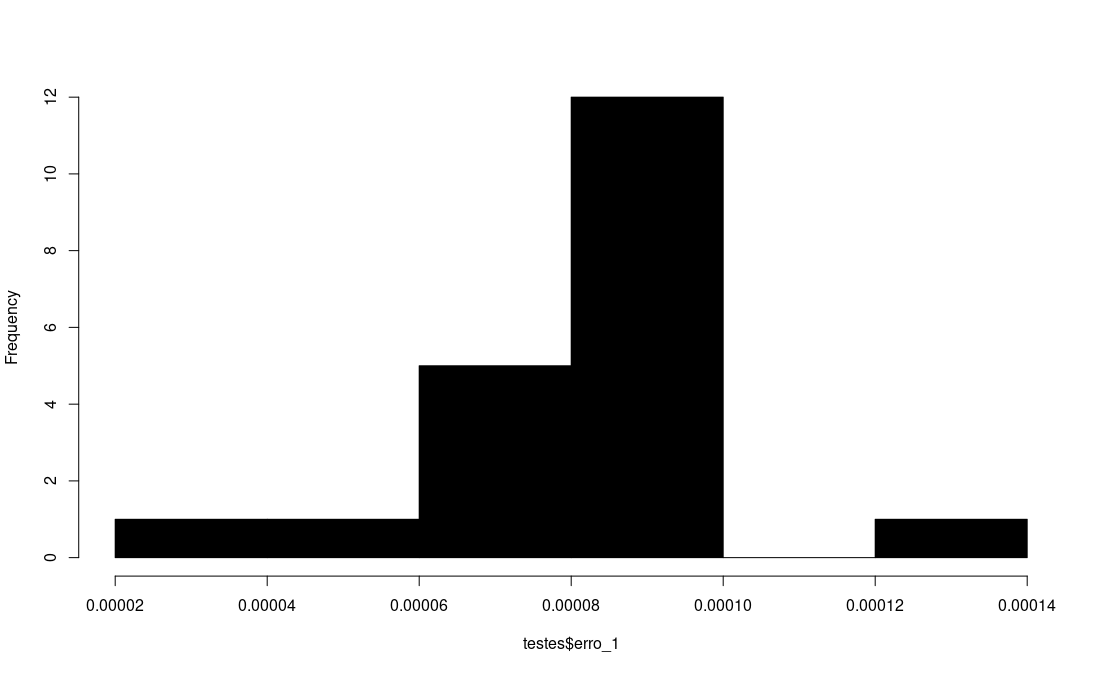
\includegraphics[scale=0.4]{images/histo1.png}
  \label{fig:histo1}
\end{figure}

Seguindo a análise dos testes, foi realizado um teste ANOVA com a amostra de dados coletada. O objetivo foi avaliar a variância dos dados em cada ponto e entre eles, analisando se estes diferem estatisticamente entre si. Com esta análise, obteve-se um $\rho$-valor de 0.6912, com isso tem-se embasamento estatístico para afirmar que os dados no ponto "A" e no ponto "B" são estatisticamente iguais, os erros de pose apresentados nos dois pontos não diferem entre si. Está análise pode ser visualizada na figura \ref*{fig:box1}. 

\begin{figure}[h!]
  \caption{Boxplot do conjunto de dados sem detecção da \textit{tag}.}
  \centering
  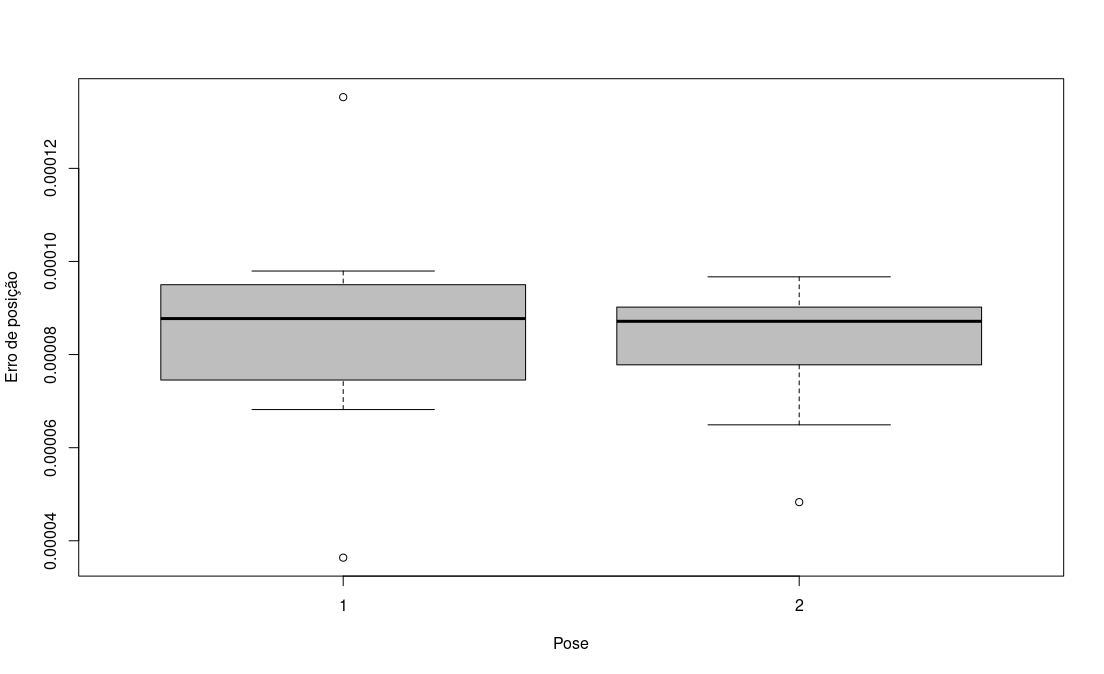
\includegraphics[scale=0.4]{images/box1.png}
  \label{fig:box1}
\end{figure}

Observando a figura \ref*{fig:box1} a pose 1 (A) possui maior variação dos seus dados em relação a pose 2 (B), porém as duas não diferem estatisticamente entre si. 

\subsubsection{Análse de variância com detecção da \textit{tag}}

Foi tomado um novo conjunto de dados, como mostra a tabela \ref*{tab:anova2}. Este experimento foi realizado com variação do operador e posição da caixa. Foram tomados dados de tempo de busca da \textit{tag}, tempo total da missão e o erro de posição do \textit{end-effector}. Também foi observado a porcentagem de sucesso na conclusão da missão, sendo o índice '1' correspondente ao sucesso na missão e o índice '-1' correspondente à falha. 

\begin{table}[H]
  \centering
  \caption{Resultados dos experimentos sem detecção da \textit{tag}.}
  \scalebox{0.8}{%
  \begin{tabular}{r|c|c|c|c|c|c|}
    \cline{2-7}
    \rowcolor[HTML]{EFEFEF} 
    \multicolumn{1}{l|}{\cellcolor[HTML]{EFEFEF}} & \textbf{Operador} & \textbf{Pose} & \textbf{Erro de pose} & \textbf{Tempo de busca} & \textbf{Tempo total} & \textbf{\begin{tabular}[c]{@{}c@{}}Sucesso\\ da missão\end{tabular}} \\ \hline
    \rowcolor[HTML]{FFFFFF} 
    \multicolumn{1}{|r|}{\cellcolor[HTML]{FFFFFF}\textbf{1}} & 1 & A & 0.010451819 & 27.1022 & 93.9316 & 1 \\ \hline
    \rowcolor[HTML]{EFEFEF} 
    \multicolumn{1}{|r|}{\cellcolor[HTML]{EFEFEF}\textbf{2}} & 1 & A & 0.009745817 & 29.1912 & 91.8192 & 1 \\ \hline
    \rowcolor[HTML]{FFFFFF} 
    \multicolumn{1}{|r|}{\cellcolor[HTML]{FFFFFF}\textbf{3}} & 1 & A & 0.010017589 & 27.3904 & 95.6437 & 1 \\ \hline
    \rowcolor[HTML]{EFEFEF} 
    \multicolumn{1}{|r|}{\cellcolor[HTML]{EFEFEF}\textbf{4}} & 1 & A & 0.010819201 & 28.4745 & 90.5214 & 1 \\ \hline
    \rowcolor[HTML]{FFFFFF} 
    \multicolumn{1}{|r|}{\cellcolor[HTML]{FFFFFF}\textbf{5}} & 1 & A & 0.011133634 & 27.7250 & 98.7845 & 1 \\ \hline
    \rowcolor[HTML]{EFEFEF} 
    \multicolumn{1}{|r|}{\cellcolor[HTML]{EFEFEF}\textbf{6}} & 1 & A & 0.010562436 & 28.8388 & 94.6226 & 1 \\ \hline
    \rowcolor[HTML]{FFFFFF} 
    \multicolumn{1}{|r|}{\cellcolor[HTML]{FFFFFF}\textbf{7}} & 1 & A & 0.010132297 & 29.1519 & 101.8420 & 1 \\ \hline
    \rowcolor[HTML]{EFEFEF} 
    \multicolumn{1}{|r|}{\cellcolor[HTML]{EFEFEF}\textbf{8}} & 1 & A & 0.010693537 & 30.2186 & 90.1885 & 1 \\ \hline
    \rowcolor[HTML]{FFFFFF} 
    \multicolumn{1}{|r|}{\cellcolor[HTML]{FFFFFF}\textbf{9}} & 2 & A & 0.010905047 & 30.2317 & 94.0104 & 1 \\ \hline
    \rowcolor[HTML]{EFEFEF} 
    \multicolumn{1}{|r|}{\cellcolor[HTML]{EFEFEF}\textbf{10}} & 2 & A & 0.010469991 & 28.9793 & 96.2312 & 1 \\ \hline
    \rowcolor[HTML]{FFFFFF} 
    \multicolumn{1}{|r|}{\cellcolor[HTML]{FFFFFF}\textbf{11}} & 2 & A & 0.010355747 & 29.0720 & 103.6160 & 1 \\ \hline
    \rowcolor[HTML]{EFEFEF} 
    \multicolumn{1}{|r|}{\cellcolor[HTML]{EFEFEF}\textbf{12}} & 2 & A & 0.010268870 & 28.6952 & 93.0651 & 1 \\ \hline
    \rowcolor[HTML]{FFFFFF} 
    \multicolumn{1}{|r|}{\cellcolor[HTML]{FFFFFF}\textbf{13}} & 2 & A & 0.010230915 & 28.6420 & 87.2120 & 1 \\ \hline
    \rowcolor[HTML]{EFEFEF} 
    \multicolumn{1}{|r|}{\cellcolor[HTML]{EFEFEF}\textbf{14}} & 2 & A & 0.004079350 & 26.8585 & 86.4156 & 1 \\ \hline
    \rowcolor[HTML]{FFFFFF} 
    \multicolumn{1}{|r|}{\cellcolor[HTML]{FFFFFF}\textbf{15}} & 2 & A & 0.004427968 & 26.1808 & 85.7109 & 1 \\ \hline
    \rowcolor[HTML]{EFEFEF} 
    \multicolumn{1}{|r|}{\cellcolor[HTML]{EFEFEF}\textbf{16}} & 2 & A & 0.009985857 & 30.0858 & 90.4296 & 1 \\ \hline
    \rowcolor[HTML]{FFFFFF} 
    \multicolumn{1}{|r|}{\cellcolor[HTML]{FFFFFF}\textbf{17}} & 1 & A & 0.009754491 & 28.2042 & 86.8758 & 1 \\ \hline
    \rowcolor[HTML]{EFEFEF} 
    \multicolumn{1}{|r|}{\cellcolor[HTML]{EFEFEF}\textbf{18}} & 1 & A & 0.010334966 & 28.6983 & 92.2869 & 1 \\ \hline
    \rowcolor[HTML]{FFFFFF} 
    \multicolumn{1}{|r|}{\cellcolor[HTML]{FFFFFF}\textbf{19}} & 1 & A & 0.010058060 & 29.4320 & 94.3545 & 1 \\ \hline
    \rowcolor[HTML]{EFEFEF} 
    \multicolumn{1}{|r|}{\cellcolor[HTML]{EFEFEF}\textbf{20}} & 1 & A & 0.010153228 & 28.1812 & 90.6696 & 1 \\ \hline
    \rowcolor[HTML]{FFFFFF} 
    \multicolumn{1}{|r|}{\cellcolor[HTML]{FFFFFF}\textbf{21}} & 1 & A & 0.010120659 & 29.2442 & 87.1852 & 1 \\ \hline
    \rowcolor[HTML]{EFEFEF} 
    \multicolumn{1}{|r|}{\cellcolor[HTML]{EFEFEF}\textbf{22}} & 1 & A & 0.010105795 & 28.9948 & 88.3569 & 1 \\ \hline
    \rowcolor[HTML]{FFFFFF} 
    \multicolumn{1}{|r|}{\cellcolor[HTML]{FFFFFF}\textbf{23}} & 1 & A & 0.010105795 & 28.9948 & 88.3569 & -1 \\ \hline
    \rowcolor[HTML]{EFEFEF} 
    \multicolumn{1}{|r|}{\cellcolor[HTML]{EFEFEF}\textbf{24}} & 1 & A & 0.011557242 & 32.9496 & 102.3640 & 1 \\ \hline
    \rowcolor[HTML]{FFFFFF} 
    \multicolumn{1}{|r|}{\cellcolor[HTML]{FFFFFF}\textbf{25}} & 2 & A & 0.011245238 & 34.7259 & 98.7636 & 1 \\ \hline
    \rowcolor[HTML]{EFEFEF} 
    \multicolumn{1}{|r|}{\cellcolor[HTML]{EFEFEF}\textbf{26}} & 2 & A & 0.011190817 & 31.1780 & 113.0500 & 1 \\ \hline
    \rowcolor[HTML]{FFFFFF} 
    \multicolumn{1}{|r|}{\cellcolor[HTML]{FFFFFF}\textbf{27}} & 2 & A & 0.010174117 & 28.7923 & 88.9735 & 1 \\ \hline
    \rowcolor[HTML]{EFEFEF} 
    \multicolumn{1}{|r|}{\cellcolor[HTML]{EFEFEF}\textbf{28}} & 2 & A & 0.010007278 & 28.8178 & 91.8702 & 1 \\ \hline
    \rowcolor[HTML]{FFFFFF} 
    \multicolumn{1}{|r|}{\cellcolor[HTML]{FFFFFF}\textbf{29}} & 2 & A & 0.009963924 & 29.0347 & 86.7183 & 1 \\ \hline
    \rowcolor[HTML]{EFEFEF} 
    \multicolumn{1}{|r|}{\cellcolor[HTML]{EFEFEF}\textbf{30}} & 2 & A & 0.010475097 & 28.2422 & 99.1881 & 1 \\ \hline
    \rowcolor[HTML]{FFFFFF} 
    \multicolumn{1}{|r|}{\cellcolor[HTML]{FFFFFF}\textbf{31}} & 2 & A & 0.010741058 & 28.2118 & 91.7459 & 1 \\ \hline
    \rowcolor[HTML]{EFEFEF} 
    \multicolumn{1}{|r|}{\cellcolor[HTML]{EFEFEF}\textbf{32}} & 2 & A & 0.004469904 & 28.4826 & 88.1583 & -1 \\ \hline
    \rowcolor[HTML]{FFFFFF} 
    \multicolumn{1}{|r|}{\cellcolor[HTML]{FFFFFF}\textbf{33}} & 1 & A & 0.010086673 & 28.7112 & 87.9372 & 1 \\ \hline
    \rowcolor[HTML]{EFEFEF} 
    \multicolumn{1}{|r|}{\cellcolor[HTML]{EFEFEF}\textbf{34}} & 1 & A & 0.010515376 & 28.8792 & 92.9002 & 1 \\ \hline
    \rowcolor[HTML]{FFFFFF} 
    \multicolumn{1}{|r|}{\cellcolor[HTML]{FFFFFF}\textbf{35}} & 1 & A & 0.010062717 & 29.1420 & 91.5910 & 1 \\ \hline
    \rowcolor[HTML]{EFEFEF} 
    \multicolumn{1}{|r|}{\cellcolor[HTML]{EFEFEF}\textbf{36}} & 1 & A & 0.010422717 & 29.0783 & 94.3296 & 1 \\ \hline
    \rowcolor[HTML]{FFFFFF} 
    \multicolumn{1}{|r|}{\cellcolor[HTML]{FFFFFF}\textbf{37}} & 1 & A & 0.010185682 & 27.9274 & 88.6971 & 1 \\ \hline
    \rowcolor[HTML]{EFEFEF} 
    \multicolumn{1}{|r|}{\cellcolor[HTML]{EFEFEF}\textbf{38}} & 1 & A & 0.010281946 & 29.7805 & 100.1800 & 1 \\ \hline
    \rowcolor[HTML]{FFFFFF} 
    \multicolumn{1}{|r|}{\cellcolor[HTML]{FFFFFF}\textbf{39}} & 1 & A & 0.013133281 & 20.0540 & 82.3651 & -1 \\ \hline
    \rowcolor[HTML]{EFEFEF} 
    \multicolumn{1}{|r|}{\cellcolor[HTML]{EFEFEF}\textbf{40}} & 1 & A & 0.012344603 & 19.1706 & 81.7740 & 1 \\ \hline

    \end{tabular}}
    \label{tab:anova2}
    % \legend{Fonte: Autoria própria.}
  \end{table}

\begin{table}[H]
    \centering
    \scalebox{0.8}{%
    \begin{tabular}{r|c|c|c|c|c|c|}
      \rowcolor[HTML]{EFEFEF} 
      \multicolumn{1}{l|}{\cellcolor[HTML]{EFEFEF}} & \textbf{Operador} & \textbf{Pose} & \textbf{Erro de pose} & \textbf{Tempo de busca} & \textbf{Tempo total} & \textbf{\begin{tabular}[c]{@{}c@{}}Sucesso\\ da missão\end{tabular}} \\ \hline
      \rowcolor[HTML]{FFFFFF} 
      \multicolumn{1}{|r|}{\cellcolor[HTML]{FFFFFF}\textbf{41}} & 2 & B & 0.005245180 & 20.4070 & 84.7338 & 1 \\ \hline
      \rowcolor[HTML]{EFEFEF} 
      \multicolumn{1}{|r|}{\cellcolor[HTML]{EFEFEF}\textbf{42}} & 2 & B & 0.007158873 & 20.4408 & 84.3043 & 1 \\ \hline
      \rowcolor[HTML]{FFFFFF} 
      \multicolumn{1}{|r|}{\cellcolor[HTML]{FFFFFF}\textbf{43}} & 2 & B & 0.011482759 & 20.7824 & 83.2411 & 1 \\ \hline
      \rowcolor[HTML]{EFEFEF} 
      \multicolumn{1}{|r|}{\cellcolor[HTML]{EFEFEF}\textbf{44}} & 2 & B & 0.087866430 & 23.4152 & 87.9248 & -1 \\ \hline
      \rowcolor[HTML]{FFFFFF} 
      \multicolumn{1}{|r|}{\cellcolor[HTML]{FFFFFF}\textbf{45}} & 2 & B & 0.008514302 & 19.9797 & 86.4344 & 1 \\ \hline
      \rowcolor[HTML]{EFEFEF} 
      \multicolumn{1}{|r|}{\cellcolor[HTML]{EFEFEF}\textbf{46}} & 2 & B & 0.005144988 & 19.8502 & 84.5138 & 1 \\ \hline
      \rowcolor[HTML]{FFFFFF} 
      \multicolumn{1}{|r|}{\cellcolor[HTML]{FFFFFF}\textbf{47}} & 2 & B & 0.013200185 & 19.9392 & 85.7667 & -1 \\ \hline
      \rowcolor[HTML]{EFEFEF} 
      \multicolumn{1}{|r|}{\cellcolor[HTML]{EFEFEF}\textbf{48}} & 2 & B & 0.004874412 & 20.2860 & 80.6176 & 1 \\ \hline
      \rowcolor[HTML]{FFFFFF} 
      \multicolumn{1}{|r|}{\cellcolor[HTML]{FFFFFF}\textbf{49}} & 1 & B & 0.012512453 & 20.7894 & 85.9667 & 1 \\ \hline
      \rowcolor[HTML]{EFEFEF} 
      \multicolumn{1}{|r|}{\cellcolor[HTML]{EFEFEF}\textbf{50}} & 1 & B & 0.014427715 & 19.4977 & 81.7383 & -1 \\ \hline
      \rowcolor[HTML]{FFFFFF} 
      \multicolumn{1}{|r|}{\cellcolor[HTML]{FFFFFF}\textbf{51}} & 1 & B & 0.007453902 & 20.5577 & 82.4847 & 1 \\ \hline
      \rowcolor[HTML]{EFEFEF} 
      \multicolumn{1}{|r|}{\cellcolor[HTML]{EFEFEF}\textbf{52}} & 1 & B & 0.006078841 & 20.4143 & 81.6851 & 1 \\ \hline
      \rowcolor[HTML]{FFFFFF} 
      \multicolumn{1}{|r|}{\cellcolor[HTML]{FFFFFF}\textbf{53}} & 1 & B & 0.009550672 & 19.5227 & 84.7312 & 1 \\ \hline
      \rowcolor[HTML]{EFEFEF} 
      \multicolumn{1}{|r|}{\cellcolor[HTML]{EFEFEF}\textbf{54}} & 1 & B & 0.006123619 & 16.9920 & 74.6466 & 1 \\ \hline
      \rowcolor[HTML]{FFFFFF} 
      \multicolumn{1}{|r|}{\cellcolor[HTML]{FFFFFF}\textbf{55}} & 1 & B & 0.003705978 & 18.6949 & 80.1175 & 1 \\ \hline
      \rowcolor[HTML]{EFEFEF} 
      \multicolumn{1}{|r|}{\cellcolor[HTML]{EFEFEF}\textbf{56}} & 1 & B & 0.006896455 & 19.9972 & 76.2407 & 1 \\ \hline
      \rowcolor[HTML]{FFFFFF} 
      \multicolumn{1}{|r|}{\cellcolor[HTML]{FFFFFF}\textbf{57}} & 2 & B & 0.006869856 & 18.8696 & 79.7714 & 1 \\ \hline
      \rowcolor[HTML]{EFEFEF} 
      \multicolumn{1}{|r|}{\cellcolor[HTML]{EFEFEF}\textbf{58}} & 2 & B & 0.002917472 & 18.4679 & 73.9755 & 1 \\ \hline
      \rowcolor[HTML]{FFFFFF} 
      \multicolumn{1}{|r|}{\cellcolor[HTML]{FFFFFF}\textbf{59}} & 2 & B & 0.004802752 & 19.4849 & 80.2423 & 1 \\ \hline
      \rowcolor[HTML]{EFEFEF} 
      \multicolumn{1}{|r|}{\cellcolor[HTML]{EFEFEF}\textbf{60}} & 2 & B & 0.004557056 & 19.5606 & 77.7174 & 1 \\ \hline
      \rowcolor[HTML]{FFFFFF} 
      \multicolumn{1}{|r|}{\cellcolor[HTML]{FFFFFF}\textbf{61}} & 2 & B & 0.006353444 & 18.5702 & 76.3386 & 1 \\ \hline
      \rowcolor[HTML]{EFEFEF} 
      \multicolumn{1}{|r|}{\cellcolor[HTML]{EFEFEF}\textbf{62}} & 2 & B & 0.007120232 & 19.6487 & 78.9122 & 1 \\ \hline
      \rowcolor[HTML]{FFFFFF} 
      \multicolumn{1}{|r|}{\cellcolor[HTML]{FFFFFF}\textbf{63}} & 2 & B & 0.004832266 & 17.0441 & 77.3120 & 1 \\ \hline
      \rowcolor[HTML]{EFEFEF} 
      \multicolumn{1}{|r|}{\cellcolor[HTML]{EFEFEF}\textbf{64}} & 2 & B & 0.004535360 & 18.0856 & 77.5731 & 1 \\ \hline
      \rowcolor[HTML]{FFFFFF} 
      \multicolumn{1}{|r|}{\cellcolor[HTML]{FFFFFF}\textbf{65}} & 1 & B & 0.007897063 & 17.1585 & 78.1917 & 1 \\ \hline
      \rowcolor[HTML]{EFEFEF} 
      \multicolumn{1}{|r|}{\cellcolor[HTML]{EFEFEF}\textbf{66}} & 1 & B & 0.007330963 & 20.5918 & 81.1574 & 1 \\ \hline
      \rowcolor[HTML]{FFFFFF} 
      \multicolumn{1}{|r|}{\cellcolor[HTML]{FFFFFF}\textbf{67}} & 1 & B & 0.008284862 & 20.2515 & 79.0624 & 1 \\ \hline
      \rowcolor[HTML]{EFEFEF} 
      \multicolumn{1}{|r|}{\cellcolor[HTML]{EFEFEF}\textbf{68}} & 1 & B & 0.008096144 & 19.9652 & 81.4914 & 1 \\ \hline
      \rowcolor[HTML]{FFFFFF} 
      \multicolumn{1}{|r|}{\cellcolor[HTML]{FFFFFF}\textbf{69}} & 1 & B & 0.013425916 & 19.0627 & 79.8650 & -1 \\ \hline
      \rowcolor[HTML]{EFEFEF} 
      \multicolumn{1}{|r|}{\cellcolor[HTML]{EFEFEF}\textbf{70}} & 1 & B & 0.007966466 & 18.6261 & 75.1340 & 1 \\ \hline
      \rowcolor[HTML]{FFFFFF} 
      \multicolumn{1}{|r|}{\cellcolor[HTML]{FFFFFF}\textbf{71}} & 1 & B & 0.008486843 & 18.1093 & 72.8817 & 1 \\ \hline
      \rowcolor[HTML]{EFEFEF} 
      \multicolumn{1}{|r|}{\cellcolor[HTML]{EFEFEF}\textbf{72}} & 1 & B & 0.007759457 & 18.7750 & 77.1361 & 1 \\ \hline
      \rowcolor[HTML]{FFFFFF} 
      \multicolumn{1}{|r|}{\cellcolor[HTML]{FFFFFF}\textbf{73}} & 2 & B & 0.012489658 & 20.1018 & 77.2422 & 1 \\ \hline
      \rowcolor[HTML]{EFEFEF} 
      \multicolumn{1}{|r|}{\cellcolor[HTML]{EFEFEF}\textbf{74}} & 2 & B & 0.008122309 & 18.6224 & 77.0045 & 1 \\ \hline
      \rowcolor[HTML]{FFFFFF} 
      \multicolumn{1}{|r|}{\cellcolor[HTML]{FFFFFF}\textbf{75}} & 2 & B & 0.012097601 & 20.3431 & 79.8706 & 1 \\ \hline
      \rowcolor[HTML]{EFEFEF} 
      \multicolumn{1}{|r|}{\cellcolor[HTML]{EFEFEF}\textbf{76}} & 2 & B & 0.087776215 & 17.5113 & 77.7186 & 1 \\ \hline
      \rowcolor[HTML]{FFFFFF} 
      \multicolumn{1}{|r|}{\cellcolor[HTML]{FFFFFF}\textbf{77}} & 2 & B & 0.006999748 & 17.3791 & 74.1548 & 1 \\ \hline
      \rowcolor[HTML]{EFEFEF} 
      \multicolumn{1}{|r|}{\cellcolor[HTML]{EFEFEF}\textbf{78}} & 2 & B & 0.008223493 & 18.3666 & 76.5340 & 1 \\ \hline
      \rowcolor[HTML]{FFFFFF} 
      \multicolumn{1}{|r|}{\cellcolor[HTML]{FFFFFF}\textbf{79}} & 2 & B & 0.008721295 & 19.4229 & 73.9818 & 1 \\ \hline
      \rowcolor[HTML]{EFEFEF} 
      \multicolumn{1}{|r|}{\cellcolor[HTML]{EFEFEF}\textbf{80}} & 2 & B & 0.008375202 & 18.6691 & 73.7671 & 1 \\ \hline
    \end{tabular}}
    \legend{Fonte: Autoria própria.}
\end{table}

Observando a tabela \ref*{tab:anova2}, os testes apresentaram 91.25\% de sucesso, ou seja, dos 80 testes realizados, em 73 obteve-se sucesso no pressionamento do botão. A tabela \ref*{tab:resumo1} resume alguns indicadores importantes das três saídas do sistema (tempo de busca, tempo total da missão e erro de pose).

\begin{table}[h!]
  \centering
  \caption{Resumo dos conjuntos de dados das variáveis de saída.}
  \scalebox{0.9}{%
  \begin{tabular}{c|c|c|c|}
    \cline{2-4}
    \rowcolor[HTML]{EFEFEF} 
    \multicolumn{1}{l|}{\cellcolor[HTML]{FFFFFF}} & \textbf{Média} & \textbf{\begin{tabular}[c]{@{}c@{}}Desvio \\ padrão\end{tabular}} & \textbf{\begin{tabular}[c]{@{}c@{}}$\rho$-valor\\ (Shapiro-Wilk)\end{tabular}} \\ \hline
    \rowcolor[HTML]{FFFFFF} 
    \multicolumn{1}{|c|}{\cellcolor[HTML]{FFFFFF}\textbf{Tempo de busca}} & 23.95025 & 5.035711 & 1.103e-07 \\ \hline
    \rowcolor[HTML]{EFEFEF} 
    \multicolumn{1}{|c|}{\cellcolor[HTML]{EFEFEF}\textbf{Tempo total}} & 86.06149 & 8.343288 & 0.02409 \\ \hline
    \rowcolor[HTML]{FFFFFF} 
    \multicolumn{1}{|c|}{\cellcolor[HTML]{FFFFFF}\textbf{Erro de pose}} & 0.01095061 & 0.0126478 & 2.2e-16 \\ \hline
    \end{tabular}}
    \label{tab:resumo1}
    \legend{Fonte: Autoria própria.}
  \end{table}

Os testes de normalidade apresentaram valores de $\rho$-valor inferiores a 0.05, ou seja, a hipótese nula não pode ser rejeitada, logo os dados seguem uma distribuição normal. 


\begin{table}[H]
  \centering
  \caption{Tabela dos valores de $\rho$-valor do teste ANOVA. }
  \scalebox{1}{%
  \begin{tabular}{c|c|}
    \cline{2-2}
     & \cellcolor[HTML]{EFEFEF}\textbf{p-valor} \\ \hline
    \rowcolor[HTML]{FFFFFF} 
    \multicolumn{1}{|c|}{\cellcolor[HTML]{FFFFFF}\textbf{Erro de pose}} & 0.525 \\ \hline
    \rowcolor[HTML]{EFEFEF} 
    \multicolumn{1}{|c|}{\cellcolor[HTML]{EFEFEF}\textbf{Tempo de busca}} & 2.2e-16 \\ \hline
    \rowcolor[HTML]{FFFFFF} 
    \multicolumn{1}{|c|}{\cellcolor[HTML]{FFFFFF}\textbf{Tempo total}} & 2.2e-16 \\ \hline
    \end{tabular}}
    \label{tab:resumo2}
    \legend{Fonte: Autoria própria.}
  \end{table}


Realizando o teste do ANOVA, podemos visualizar a variância dos pontos A e B em relação ao erro de pose, tempo de busca e tempo total da missão. A tabela \ref*{tab:resumo2} apresenta o $\rho$-valor para cada conjunto de dados, e a partir dessa análise podemos chegar a conclusão que a hipótese nula não pode ser rejeitada para o erro de pose assim como visto na análise passada, ou seja, os dados obtidos do erro de posição do \textit{end-effector} nos pontos A e B são estatisticamente iguais. Já os dados dos tempo de busca e tempo total da missão apresentam $\rho$-valor menor que 0.05, logo a hipótese nula é rejeitada e pode-se concluir que os dados diferem entre si, como mostram os \textit{boxplots} das figuras \ref*{fig:box4} e \ref*{fig:box5}.

\begin{figure}[H]
  \caption{\textit{Boxplot} da variância do tempo de busca entre os pontos A e B. }
  \centering
  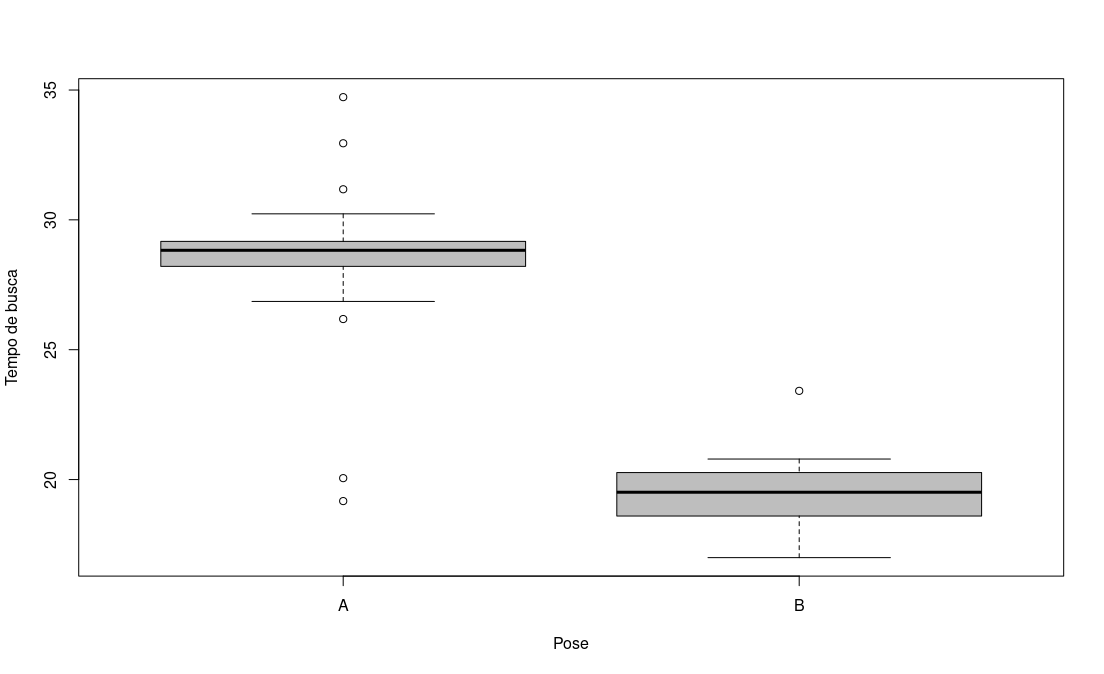
\includegraphics[scale=0.45]{images/box4_tb.png}
  \label{fig:box4}
  \legend{Fonte: Autoria própria.}
\end{figure}
\begin{figure}[H]
  \caption{\textit{Boxplot} da variância do tempo total da missão entre os pontos A e B. }
  \centering
  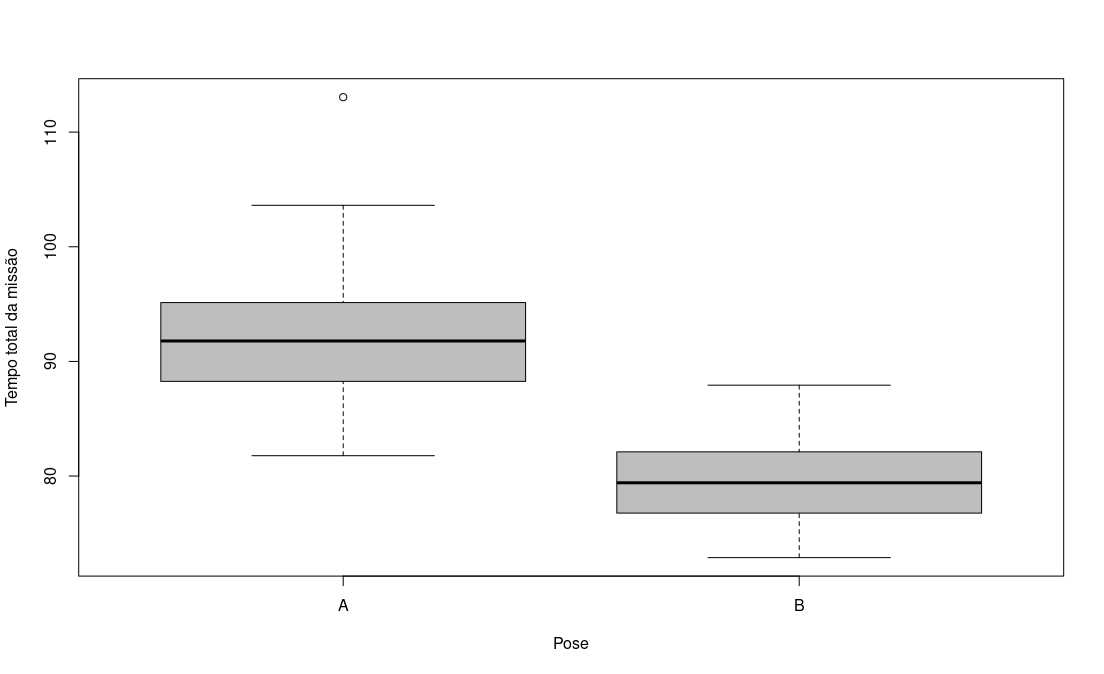
\includegraphics[scale=0.45]{images/box3_tt.png}
  \label{fig:box5}
  \legend{Fonte: Autoria própria.}
\end{figure}

% As figuras xx, yy e zz apresentadas a seguir apresentam o histograma de cada uma das variáveis e de forma visual pode-se notar a distribuição dos dados. 

% \begin{figure}[H]
%   \caption{Histograma dos erros de pose no ponto A. }
%   \centering
%   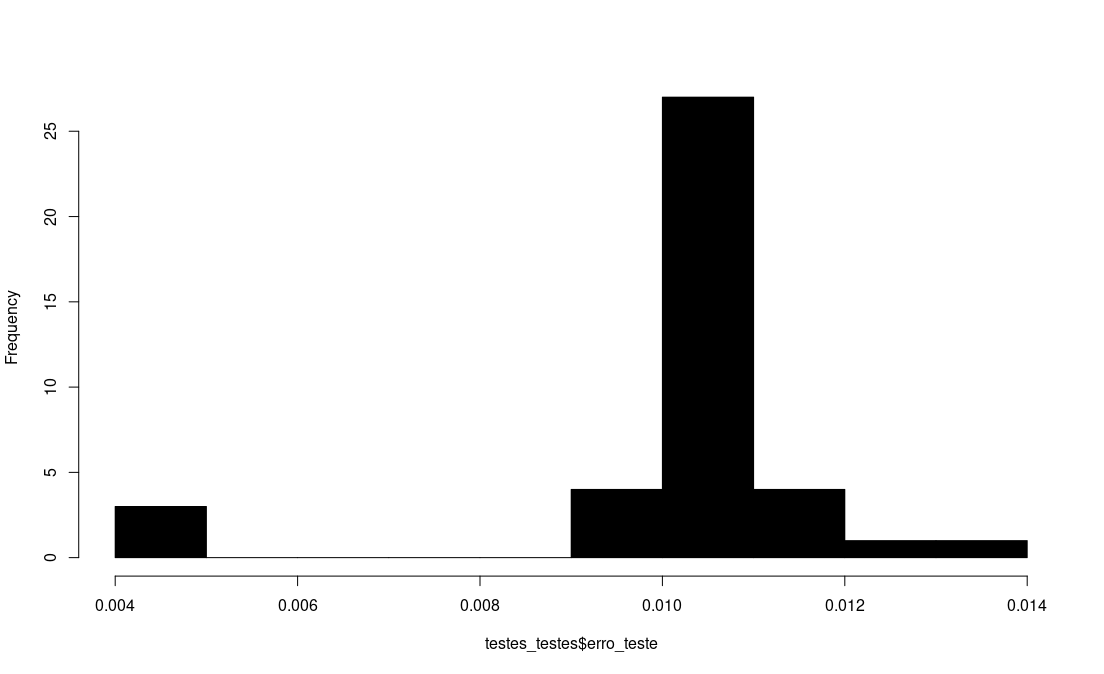
\includegraphics[scale=0.35]{images/histo2_ea.png}
%   \label{fig:histo2}
% \end{figure}
% \begin{figure}[H]
%   \caption{Histograma dos erros de pose no ponto B.}
%   \centering
%   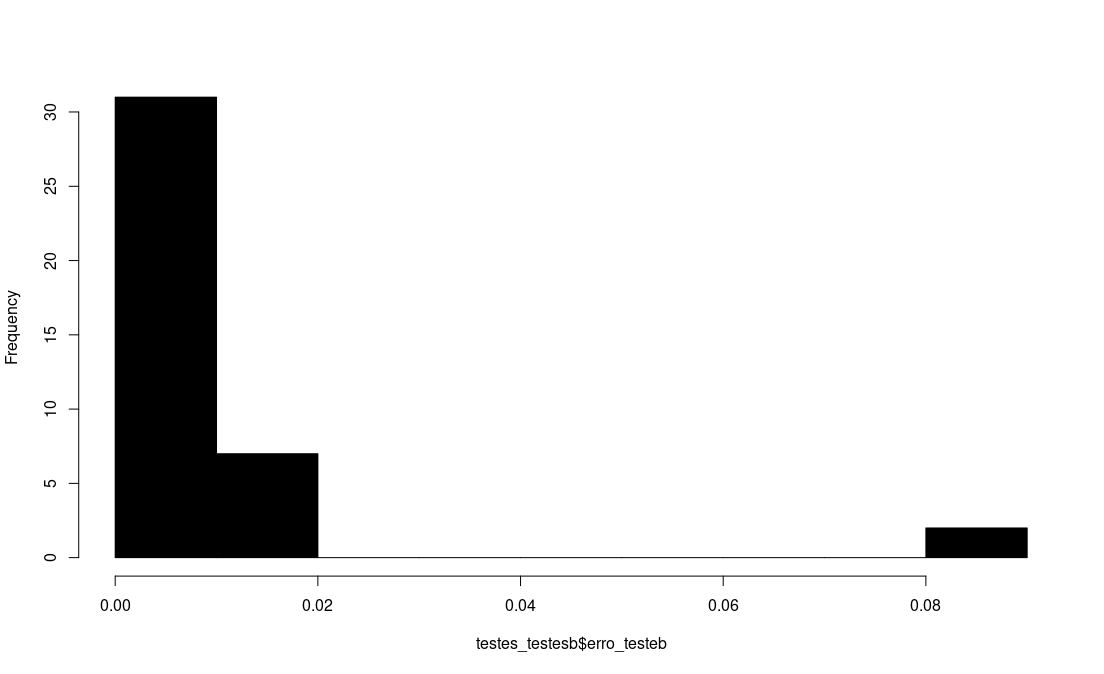
\includegraphics[scale=0.35]{images/histo3_eb.png}
%   \label{fig:histo3}
% \end{figure}
% \begin{figure}[H]
%   \caption{Histograma do tempo de busca no ponto A.}
%   \centering
%   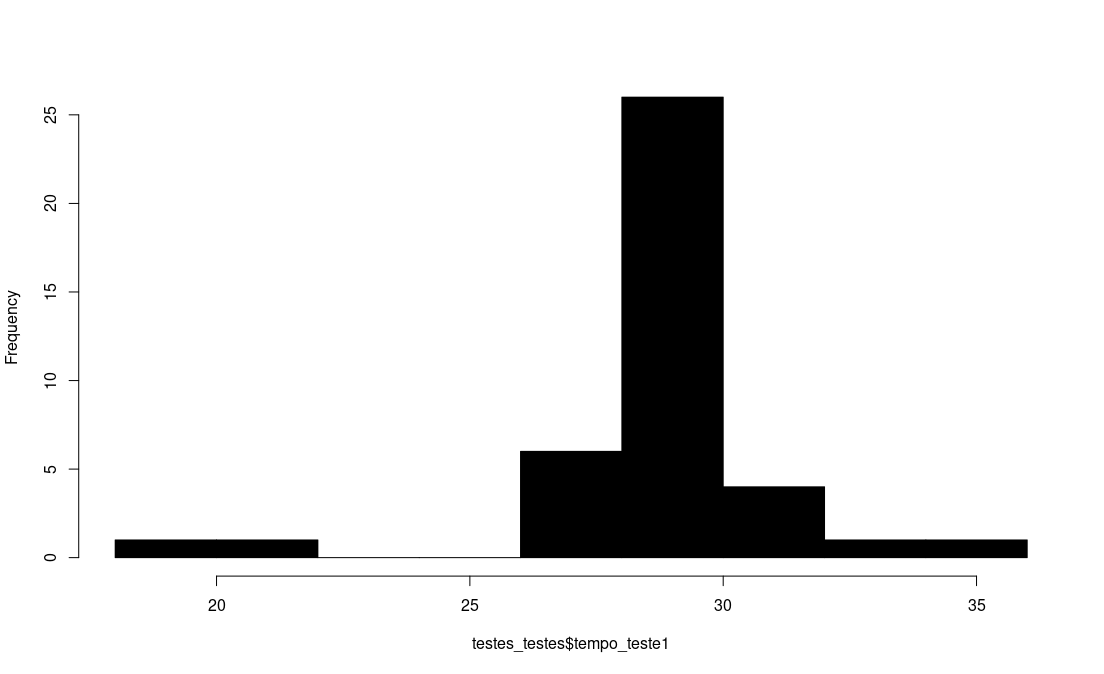
\includegraphics[scale=0.35]{images/histo_tba.png}
%   \label{fig:histo4}
% \end{figure}
% \begin{figure}[H]
%   \caption{Histograma do tempo de busca no ponto B.}
%   \centering
%   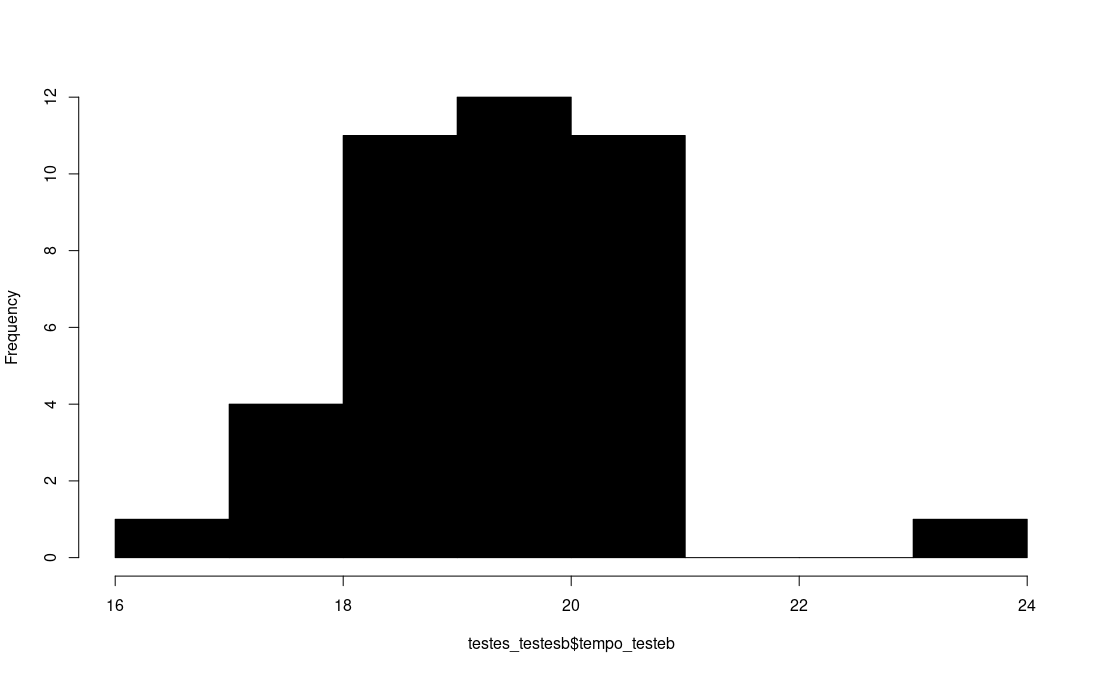
\includegraphics[scale=0.35]{images/histo_tbb.png}
%   \label{fig:histo5}
% \end{figure}
% \begin{figure}[H]
%   \caption{Histograma do tempo total da missão no ponto A.}
%   \centering
%   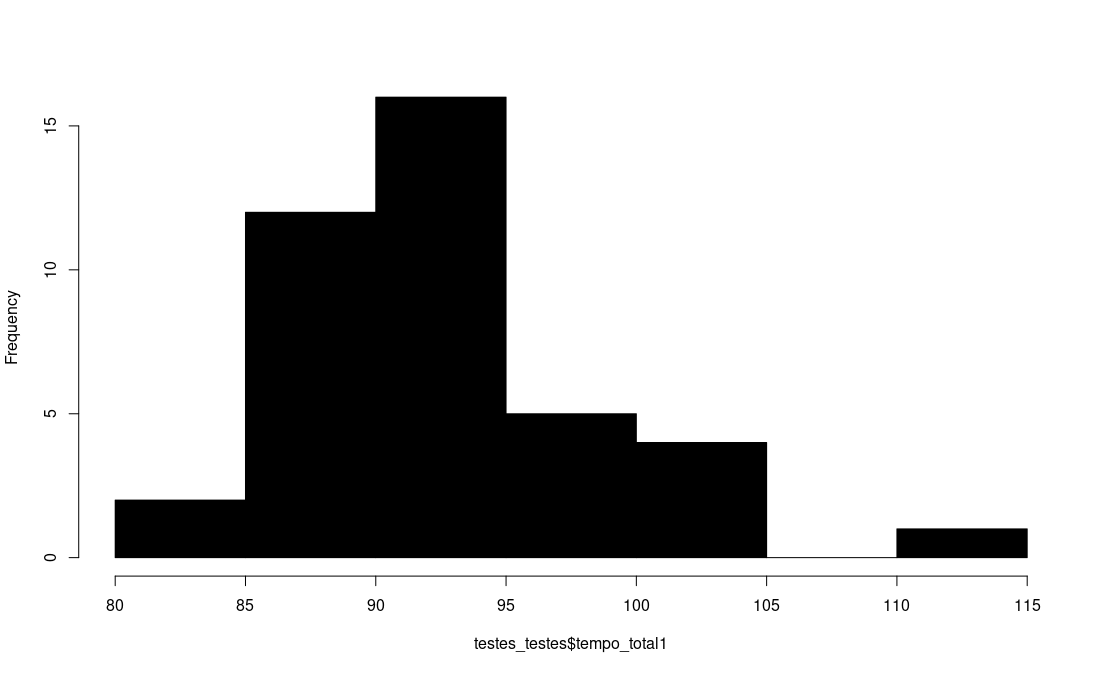
\includegraphics[scale=0.35]{images/histo_tta.png}
%   \label{fig:histo6}
% \end{figure}
% \begin{figure}[H]
%   \caption{Histograma do tempo total da missão no ponto B.}
%   \centering
%   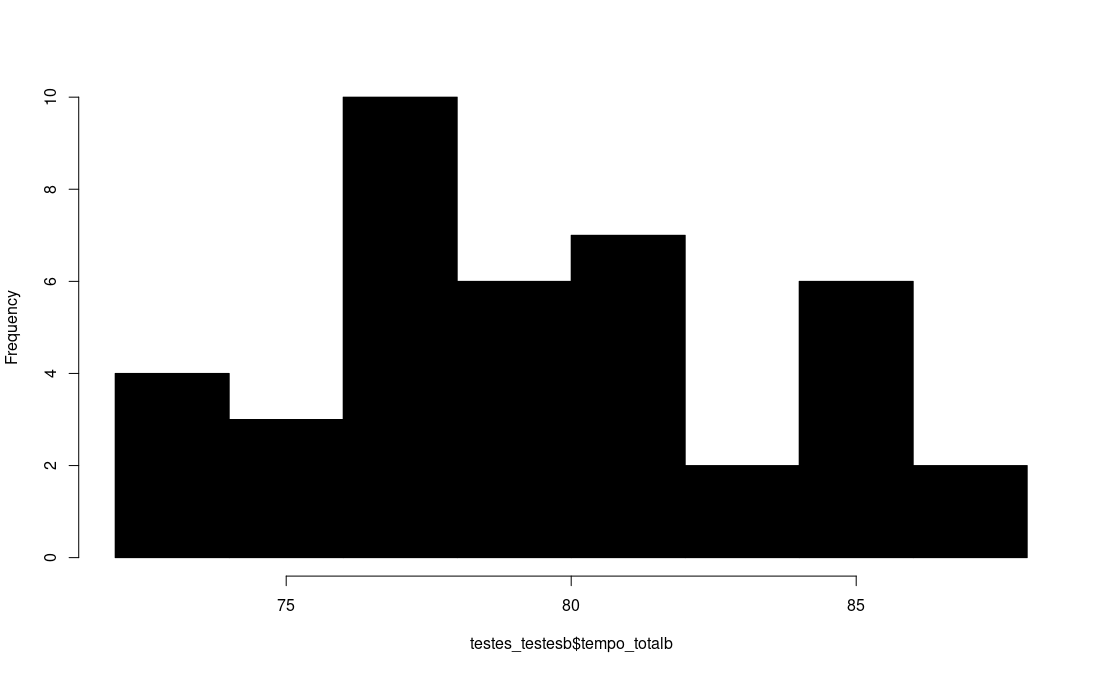
\includegraphics[scale=0.35]{images/histo_ttb.png}
%   \label{fig:histo7}
% \end{figure}


\subsection{Análise de repetibilidade e reprodutibilidade}

Como forma de avaliação do sistema robótico, também foi adotado um estudo de repetibilidade e reprodutibilidade do sistema. Com isso, foram adotados os dados da tabela \ref*{tab:anova2}. Foram tomadas 20 medições de cada operador para cada pose da caixa, totalizando 80 testes e assim foram obtidos os seguintes dados apresentados na figura \ref*{fig:rr1} e \ref*{fig:rr2}.


\begin{figure}[h!]
  \caption{Modelo completo teste R\&R para tempo de busca.}
  \centering
  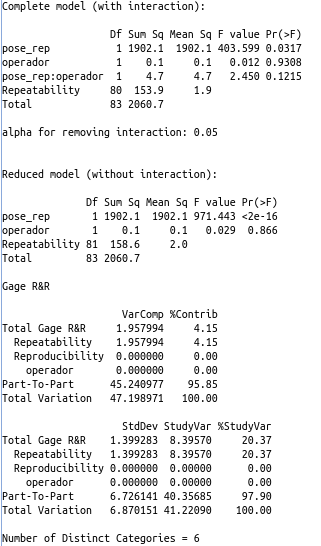
\includegraphics[scale=0.55]{images/rr_tb.png}
  \label{fig:rr1}
  \legend{Fonte: Autoria própria.}
\end{figure}

% \begin{figure}[H]
%   \caption{Modelo completo teste R\&R para tempo total da missão.}
%   \centering
%   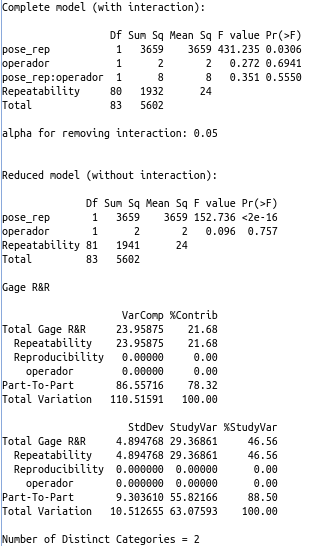
\includegraphics[scale=0.6]{images/rr_tt.png}
%   \label{fig:rr2}
%   \legend{Fonte: Autoria própria.}
% \end{figure}

Observando a figura \ref*{fig:rr1}, correspondente ao teste de R\&R para o tempo busca do marcador visual, neste teste percebe-se o número de categorias igual a 6, número considerável e acima de valores de referências, o que demonstra que o sistema de medição pode ser utilizado para análise dos dados. Outro ponto importante para observado é o indicador "\textit{Total Gage R\&R}", que foi calculado em 20.37, inferior a 30\% (Valor máximo aceitável adotado em algumas literaturas). 

O sistema sendo aceitável para análise, pode-se observar outros indicadores importantes para análise, como exemplo do $\rho$-valor, que mostra a maior influência na variação devido a pose da caixa, não ocorrendo influência do operador ou da interação entre operador e pose. O indicador "\textit{Part-to-Part}" indica que aproximadamento 98\% da variação do sistema deve-se a própria variação de pose da caixa, o que demonstra que o sistema possui repetibilidade e reprodutibilidade, quanto a variável de tempo de busca.

\begin{figure}[H]
  \caption{Modelo completo teste R\&R para tempo total da missão.}
  \centering
  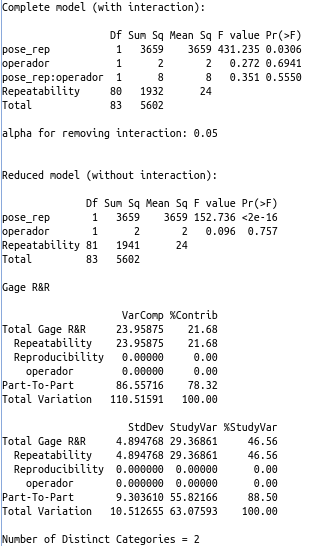
\includegraphics[scale=0.55]{images/rr_tt.png}
  \label{fig:rr2}
  \legend{Fonte: Autoria própria.}
\end{figure}

O mesmo não pode ser observado na figura \ref*{fig:rr2}, onde o número de categorias apresentados é baixo e o índice "\textit{Total Gage R\&R}" foi calculado em 46.56\%, acima do valor máximo de referência (30\%), o que mostra que o sistema de medição não é aceitável quando observado a variável de tempo total da missão.  

Seguindo a análise dos dados obtidos no estudo de repetibilidade e reprodutibilidade do sistema para o tempo de busca, visualizamos cartas na figura \ref*{fig:rr3} que possibilita um melhor entendimento do sistema de medição.

\begin{figure}[H]
  \caption{Gráficos do estudo R\&R para tempo de busca.}
  \centering
  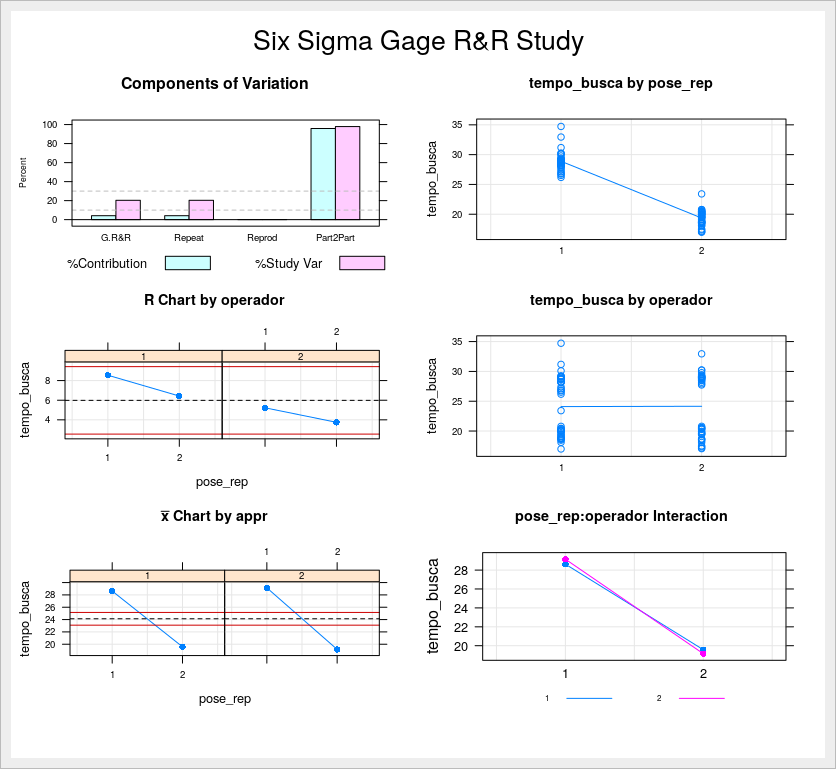
\includegraphics[scale=0.7]{images/rr_bus.png}
  \label{fig:rr3}
  \legend{Fonte: Autoria própria.}
\end{figure}

A carta "Componentes de variação" representa atribuições da variação do sistema, e como observado na figura \ref*{fig:rr3}, a variação deve-se principalmente a "peça por peça" ou "parte por parte", o que é desejável, demonstrando que o sistema de medição é aceitável para análise do tempo de busca do manipulador. 

A carta R é uma carta de controle de amplitudes que representa graficamente a consistência do operador. Os pontos apresentados na figura \ref*{fig:rr3} estão dentro dos limites máximos e mínimos, ou seja, é sinal de que os operadores estão realizando os testes de forma consistente.

Os pontos apresentados na carta Xbar, na figura \ref*{fig:rr3}, os dados estão acima ou abaixo dos limites de controle. Estes resultados indicam que a variação
entre as poses são maiores que a variação do dispositivo de medição. 

Outro ponto importante de ser destacado é o gráfico de interação entre o operador e o tempo de busca (figura \ref*{fig:rr3}), a barra horizontal visualizada, demonstra que os operadores estão realizando medições semelhantes entre si, com variações semelhantes entre as medidas máximas e mínimas do tempo de busca. 



% \begin{knitrout}
%   \begin{kframe}
%   \begin{verbatim}
%       Complete model (with interaction):

%       Df Sum Sq Mean Sq F value Pr(>F)
%   pose_rep           1   3659    3659 431.235 0.0306
%   operador           1      2       2   0.272 0.6941
%   pose_rep:operador  1      8       8   0.351 0.5550
%   Repeatability     80   1932      24               
%   Total             83   5602                       

%   alpha for removing interaction: 0.05 


%   Reduced model (without interaction):

%   Df Sum Sq Mean Sq F value Pr(>F)
%   pose_rep       1   3659    3659 152.736 <2e-16
%   operador       1      2       2   0.096  0.757
%   Repeatability 81   1941      24               
%   Total         83   5602                       

%   Gage R&R

%         VarComp %Contrib
%   Total Gage R&R     23.95875    21.68
%   Repeatability    23.95875    21.68
%   Reproducibility   0.00000     0.00
%   operador        0.00000     0.00
%   Part-To-Part       86.55716    78.32
%   Total Variation   110.51591   100.00

%         StdDev StudyVar %StudyVar
%   Total Gage R&R     4.894768 29.36861     46.56
%   Repeatability    4.894768 29.36861     46.56
%   Reproducibility  0.000000  0.00000      0.00
%   operador       0.000000  0.00000      0.00
%   Part-To-Part       9.303610 55.82166     88.50
%   Total Variation   10.512655 63.07593    100.00

%   Number of Distinct Categories = 2 
% \end{verbatim}
% \end{kframe}
% \end{knitrout}


% \begin{knitrout}
%   \begin{kframe}
%   \begin{verbatim}
%   Complete model (with interaction):

%   Df Sum Sq Mean Sq F value Pr(>F)
% pose_rep           1 1902.1  1902.1 403.599 0.0317
% operador           1    0.1     0.1   0.012 0.9308
% pose_rep:operador  1    4.7     4.7   2.450 0.1215
% Repeatability     80  153.9     1.9               
% Total             83 2060.7                       

% alpha for removing interaction: 0.05 


% Reduced model (without interaction):

% Df Sum Sq Mean Sq F value Pr(>F)
% pose_rep       1 1902.1  1902.1 971.443 <2e-16
% operador       1    0.1     0.1   0.029  0.866
% Repeatability 81  158.6     2.0               
% Total         83 2060.7                       

% Gage R&R

%     VarComp %Contrib
% Total Gage R&R     1.957994     4.15
% Repeatability    1.957994     4.15
% Reproducibility  0.000000     0.00
% operador       0.000000     0.00
% Part-To-Part      45.240977    95.85
% Total Variation   47.198971   100.00

%     StdDev StudyVar %StudyVar
% Total Gage R&R    1.399283  8.39570     20.37
% Repeatability   1.399283  8.39570     20.37
% Reproducibility 0.000000  0.00000      0.00
% operador      0.000000  0.00000      0.00
% Part-To-Part      6.726141 40.35685     97.90
% Total Variation   6.870151 41.22090    100.00

% Number of Distinct Categories = 6 
% \end{verbatim}
% \end{kframe}
% \end{knitrout}


\section{Conclusões dos testes estatísticos}

Após estudo dos dados obtidos a partir de testes no manipulador robótico, verifica-se que os dados apresentaram distribuição normal, o que possibilita uma análise confiável dos mesmos, comprovando isso através de histogramas apresentados durante a seção. 

Também é possível observar nos testes realizados que o algoritmo de planejamento de trajetória RRT CONNECT apresentou melhor resultado em relação ao Kpiece, bem como a velocidade pouco influenciou nos testes, mostrando que a melhor configuração para o sistema para as missões impostas é utilizando o algoritmo RRT. 

Não houve diferença no erro de posicionamento do \textit{end-effector} quando observado as poses A e B e com ou sem detecção do marcador visual, ou seja, pode-se concluir que o manipulador robótico apresenta erro constante nas poses analisadas. É observado também que o tempo de busca e tempo total da missão diferem entre as poses. 

Por fim, conclui-se que a análise de repetibilidade e reprodutibilidade foi positiva quando observados os dados da variável tempo de busca do marcador visual, uma vez que o sistema de medição atendeu ao teste; enquanto que para a variável tempo total da missão os resultados não foram de todo satisfatórios, indicando possíveis direções de melhoria no sistema. 

%------------------------------------------------------------------
%\section{Análise dos experimentos}
%\label{sec:doe}


%------------------------------------------------------------------
%\section{Avaliação da prontidão tecnológica}
%\label{sec:trl}

